\chapter{Prior Study}\label{cap:planificación}

\section{Introduction}
Within this chapter, the projects that have served as a basis and inspiration for the realization of this thesis are going to be addressed. There is a wide variety of topics and implementations among them, some of them may be bigger iniciatives, some others just small personal projects carried out mainly for leisure.

Finally, a comparative chart will assist in both the drawing of conclusions as well as an overview of the possible advantages, drawbacks and features regarding the different tools or projects at issue.

\section{farmOS}
farmOS\cite{farmosrepo} project consists of a web-based application for agricultural management, planning, and record keeping.

There are several aspects to be emphasised about this iniciative. See, for example, it offers modularity and scalability as it is entirely Drupal based. However, microcontrollers and IoT integration will shape the most remarkable part to us. Moreover, the fact that it is a free software project allows us not only to use and study the source code but also grants the possibility to improve and contribute to the project.

Another positive aspect to take into account is its versatility, since it is a web application, it only needs a browser to execute so it can be easily run in a bunch of different devices.

\subsection{Structure}
It is interesting to highlight the way in which farmOS is structured\cite{farmosguide} around the log concept. There exists four categories of diferent elements an administrator can create, they can be identified as the 4 W.
\begin{itemize}
	\item \textbf{log (when)} - these try to show what has happened over time, it is considered as the primary record.
	\item \textbf{asset (what)} - these could be understood as the things we are dealing with. E.g.: livestock, plants, seeds, sensors, equipment, etc.
	\item \textbf{areas (where)} - it is helpful for larger farmers that may need to use geo features.
	\item \textbf{people (who)} - different people can be added with different roles.
\end{itemize}


In the big picture, farmOS is meant to be a database for the farmer to store information about the farm. However, it is meant to be flexible and work on any scale. Whether we are talking about a very small urban vegetable garden some user might want to keep track of, or at the other side of the scale, a large farm with different managers, crops and so on.

In this way, the information starts to create a web of associations and a dataset is developed over time that, later on, will allow the information processing for searching, categorising, sorting or exporting data, depending on the needs of the user. 


\addcontentsline{toc}{subsubsection}{Example}
\subsubsection*{Example}

Say a farmer has two areas with two different assets per area to keep track of. Each asset has a log because of some actions that have been taken. Also, there is some information in relation to the area 2 which has also been stored in a log. In farmOS, this scenario could be represented aproximately as shown in the graph below.

\begin{figure}[htp]
    \centering
    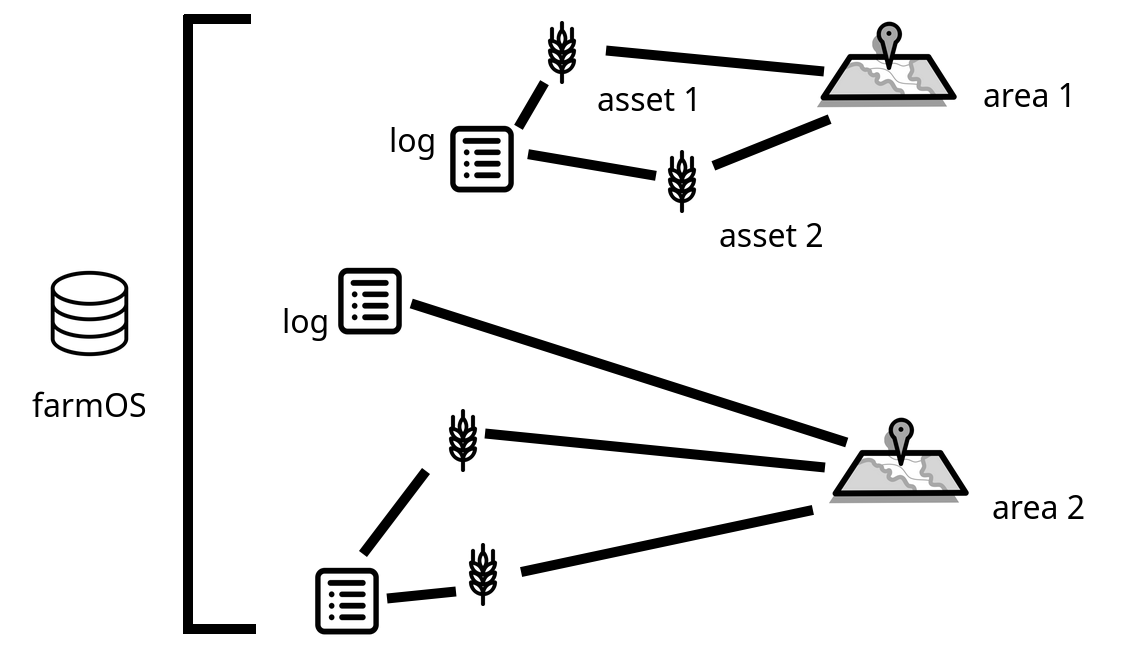
\includegraphics[width=0.75\textwidth]{fig/farmos-structure.png}
    \caption{An example of a web of associations created in farmOS dataset}
    \label{fig:farmos01}
\end{figure}


\section{Agrineer}
Continuing with this very same philosophy about building free software, there exists quite an interesting project, Agrineer. They define themselves as an open source group of computational laboratories dedicated to projects that are both practical and educational, from satellite remote sensing to down-to-earth fablabs\cite{agrineer}.

Currently, there are several tools they are working on, such as the Grow Degree Calculator (GDC) and the Soil Moisture Estimator (SME) applications.

These tools, specially the SME application, may come in handy when processing, understanding and displaying data that will be collected using sensors.


\section{Autonomous agricultural vehicles}
When technological innovation in agriculture is addressed, autonomous or driverless tractors are often one of the things that may occur to us. There is nothing new in this idea, which as been around us for about 80 years now. John Deere's autonomous tractor\cite{deere-tractor} is a good example of this kind of vehicles, that may play a key role in the not too distant future.

\begin{figure}[htp]
    \centering
    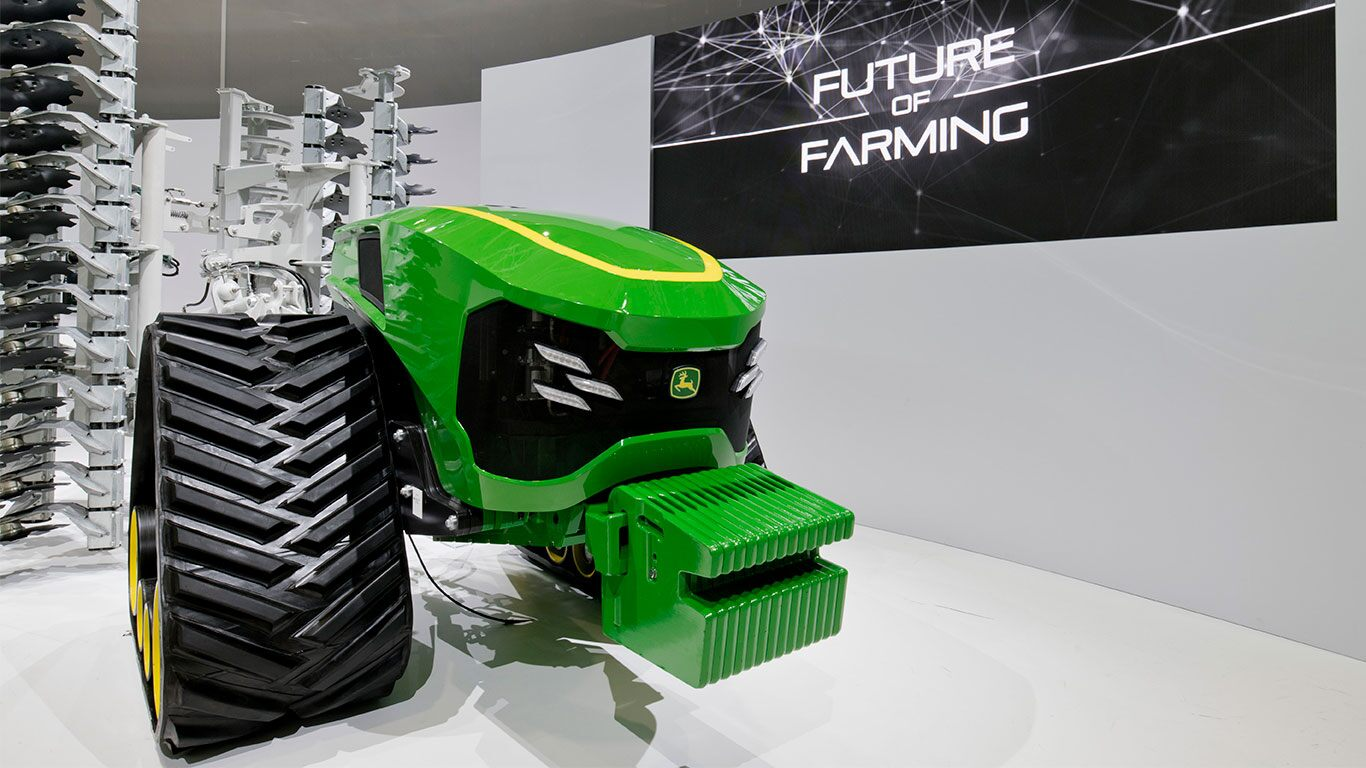
\includegraphics[width=0.75\textwidth]{fig/deere-tractor.jpg}
    \caption{John Deere’s autonomous electric tractor}
    \label{fig:deere-tractor}
\end{figure}

\subsection{PACA, a prototype agricultural vehicle}
Related to this topic, it is worth mentioning ``Computational applications in agriculture'' \cite{paca} by Carlos Gregorio Martín Pérez. In this thesis, PACA, a prototype agricultural vehicle is developed.

The main purpose of PACA is to be able to facilitate the transportation of certain elements along the property. According to the author, PACA can be controlled both remotely as well as manually. It also features a drive system capable of carrying up to 200Kg and can operate independently for about 8 hours.

\begin{figure}[htp]
    \centering
    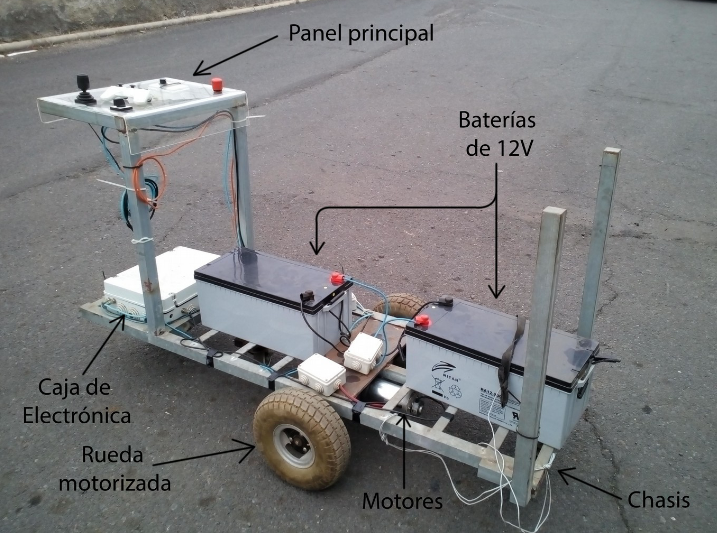
\includegraphics[width=0.5\textwidth]{fig/paca.png}
    \caption{Main components of PACA. Source: ``Computational applications in agriculture'' Bachelor's Thesis}
    \label{fig:paca}
\end{figure}

 It is some of the PACA implementation that has served as an inspiration for the development of this very own thesis, more precisely, it has caught our attention the use of the microcontroller ESP8266 in order to create a wifi network so data transmission can be allowed. Although PACA uses a Raspberry single-board computer, it is still of our interest as it can be implemented in Arduino for this same goal.

\section{Arduino controller for farming}
After mentioning some iniciatives whose objective is transform modern agriculture by introducing technological devices and solutions, we will focus now in something a bit more concrete.

As it has been mentioned before, the aim of this thesis is to be able to monitorise a garden. In order to achieve so, we need to program microcontrollers that will collect data from sensors, process it and display information or transform said data, if needed. The choices when speaking about microcontrollers are infinite, because of simplicity and the remarkable community, we are going to concentrate on Arduino.

As the reader may already be aware of, Arduino is an open-source electronics platform able to perform a wide variety of tasks: reading inputs and turn it into an output, activating a motor, turning on an LED\cite{arduino}, etc.

Among the infinitely many projects trying to achieve a similar result, the GrowBox controller project developed by Michele, in Red Sheep Labs\cite{growbox}, caught my attention as it allows configuration via server, CSV logs and uses Emoncms, this last tool was what interested me the most. As could be expected, GrowBox measures variables such as temperature, humidity, fan or lights. Emoncms is used in order to log and visualise this environmental data and it may come as a interesting asset for the further develop of this project.

\section{Comparative chart}

\begin{table}[H]
\begin{tabular}{llll}
\hline
    \rowcolor{lightpurple}
	    & \textbf{farmOS}   & \textbf{Agrineer}& \textbf{PACA} \\ \hline
    \rowcolor{lightgray}
	    feature1 & 1        & 35               & 35                              \\
	    feature2 & 1        & 3                & 3                             \\
    \rowcolor{lightgray}
	    f3       & 1        & -                & -                            \\
	    f4       & 1        & 43,95            & 43,95          \\
    \rowcolor{lightgray}
	    f5       & 5        & -                & -
\end{tabular}
\end{table}


\section{Conclusiones}
